\section{Herleitung des Algorithmus}
\label{cg:section:herleitung}
\rhead{Herleitung des Algorithmus}

\subsection{Intuition}
Die Idee des CG-Algorithmus ist, die Schwächen von Gradient Descent auszubessern.
Dies geschieht, indem pro Dimension des Minimierungsproblems nur ein Schritt benötigt wird.
Intuitiv kann man sich dies als Abstieg entlang der Koordinatenachsen vorstellen, wie in Abbildung \ref{cg:abb:koordabstieg} gezeigt.
Ein solches Verfahren findet immer in $N$ Schritten die exakte Lösung.

\begin{figure}	
	\centering
	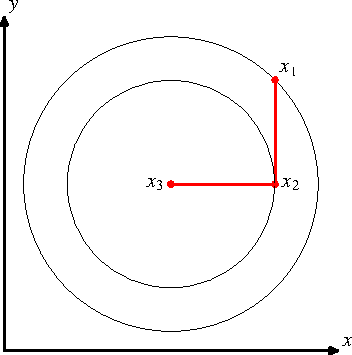
\includegraphics{papers/cg/images/descent-2}
	\caption{2D Abstieg entlang der Koordinatenachsen, 2 Schritte genügen um die exakte Lösung zu finden. 
		Abbildung aus dem Seminar Buch von 2014 \cite{cg:book:hpc}.}
	\label{cg:abb:koordabstieg}
\end{figure}

Auf den ersten Blick ist dies sehr vielversprechend.
Allerdings ist die Konvergenz dieses Verfahrens unter Umständen sehr schlecht, da die Koordinatenachsen in hochdimensionalen Problemen weit weg vom Gradienten sind.
Dabei haben viele Dimensionen keinen richtigen Einfluss und ein Abstieg in deren Richtung verbessert die Approximation nur minimal.
In Abbildung \ref{cg:abb:koordabstieg2} sieht man dieses Verhalten noch besser an einem 3D Beispiel.
Es wäre also wünschenswert einen Algorithmus zu finden, welcher:
\begin{itemize}
	\item in $N$ Schritten die exakte Lösung findet
	\item trotzdem schnell konvergiert (eine gute Approximation findet sich bereits nach weniger Schritten)
\end{itemize}
Dies wird mit dem CG-Algorithmus erreicht.

\begin{figure}	
	\centering
	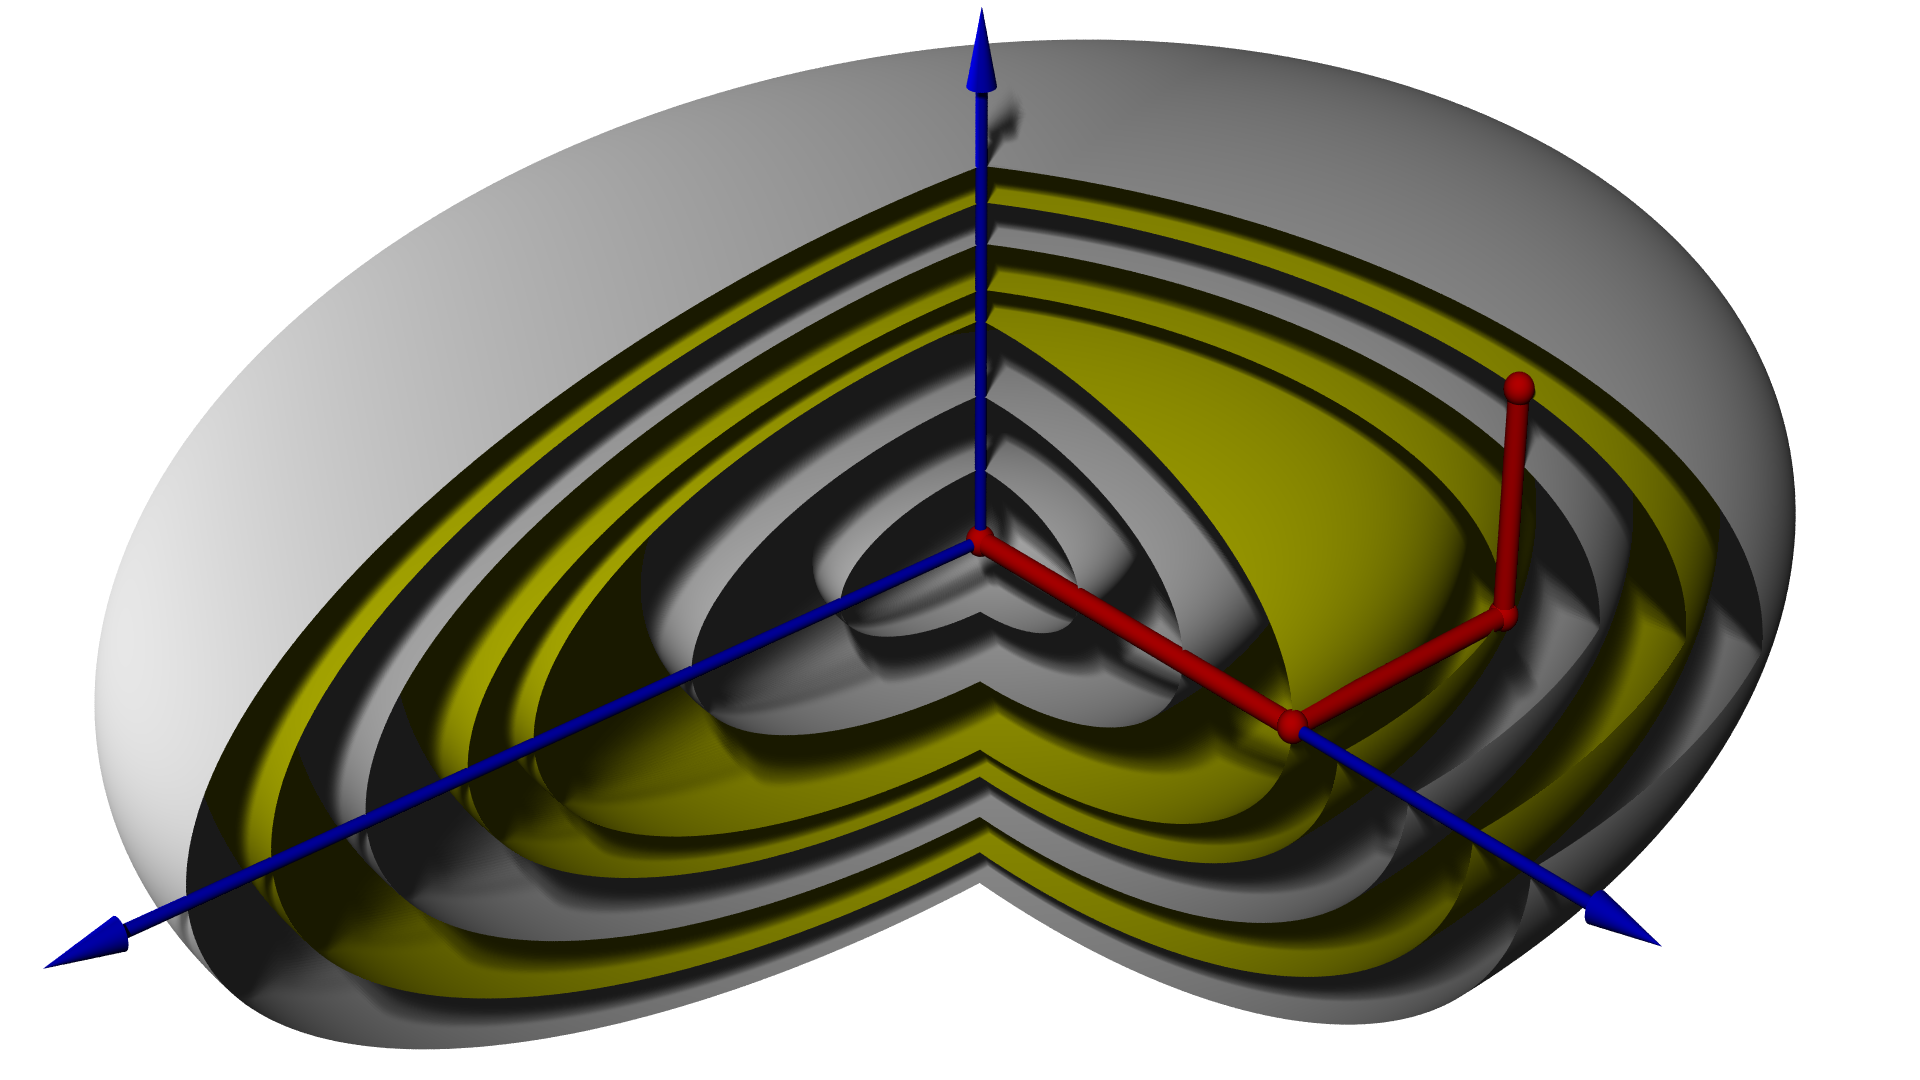
\includegraphics[width=0.8\hsize]{papers/cg/images/descent3d.jpg}
	\caption{3D Abstieg entlang der Koordinatenachsen, 3 Schritte genügen um die exakte Lösung zu finden. 
		Abbildung aus dem Seminar Buch von 2014 \cite{cg:book:hpc}.}
	\label{cg:abb:koordabstieg2}
\end{figure}



\subsection{Optimale Suchrichtung \label{cg:subsection:suchrichtung}}

Erreicht werden kann dies, indem jeweils orthogonalisierte Richtungen verwendet werden.
Kombiniert mit der optimalen Abstiegslänge aus \ref{cg:subsection:schrittweite} führt dies dazu, dass genau $N$ Schritte zur exakten Lösung führen.
Wie beim Abstieg entlang der Koordinatenachsen werden also nur neue Richtungen $d_{k+1}$ verwendet, welche orthogonal (in $A$) auf allen bisherigen Richtungen stehen
\begin{equation} 
	d_{k+1}  \perp_A  d_k  \perp_A  d_{k-1}  \dots \perp_A  d_0.
\end{equation}
Jetzt stellt sich also noch die Frage, wie diese orthogonalen Richtungen zu wählen sind um eine schnelle Konvergenz zu erreichen.
Es bietet sich wiederum der negative Gradient $r_{k+1} = b - Ax_{k+1}$ (Residuum) an, welcher danach mithilfe eines Orthogonalisierungsverfahrens orthogonalisiert werden kann.
Der negative Gradient entspricht per Definition der lokal optimalen Richtung um schnell abzusteigen und ist somit die beste Wahl.

Wir verwenden das Gram-Schmidt-Orthogonalisierungsverfahren um den Gradienten auf den bisherigen Richtungen zu orthogonalisieren.
Dabei wollen wir orthogonal in Bezug auf $A$ sein, weshalb das verallgemeinerte Skalarprodukt $\langle \dots \rangle_A$ verwendet wird 
\begin{equation}\label{cg:eq:gram}
	d_{k+1} 
	= 
	r_{k+1} - \sum_{i=0}^{k} \frac{\langle d_i , r_{k+1} \rangle_A}{\langle d_i , d_i \rangle_A} d_i.
\end{equation}
Diese vielen Orthogonalisierungen sind rechenintensiv und würden die Performance des CG-Algorithmus beeinträchtigen.
Im nächsten Abschnitt wird gezeigt, dass es genügt das Orthogonalisierungsverfahren auf der letzten Abstiegsrichtung durchzuführen.
Die neue Richtung ist dann automatisch auch auf allen vorherigen Richtungen orthogonal.
Dies führt zur folgenden, vereinfachten Berechnung
\begin{equation} 
	d_{k+1}
	= 
	r_{k+1} - \frac{\langle d_k , r_{k+1} \rangle_A}{\langle d_k , d_k \rangle_A} d_k.
\end{equation}
Abbildung \ref{cg:abb:cg1} zeigt wie in einem zweidimensionalen Problem in 2 Schritten die exakte Lösung gefunden wird und schon nach Schritt 1 eine möglichst gute Approximation erreicht wird.
Die orthogonalisierungen sind besser im dreidimensionalen Beispiel von Abbildung \ref{cg:abb:cg2} zu sehen.
Orthogonale Vektoren bezüglich $A$ werden auch als konjugiert bezeichnet, weshalb der Name konjugierte Gradienten Sinn macht.
\begin{figure}	
	\centering
	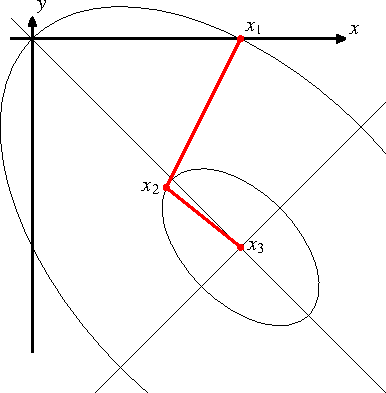
\includegraphics{papers/cg/images/descent-3}
	\caption{2D Abstieg mit dem CG-Algorithmus, 2 Schritte genügen um die exakte Lösung zu finden. 
		Abbildung aus dem Seminar Buch von 2014 \cite{cg:book:hpc}.}
	\label{cg:abb:cg1}
\end{figure}

\begin{figure}	
	\centering
	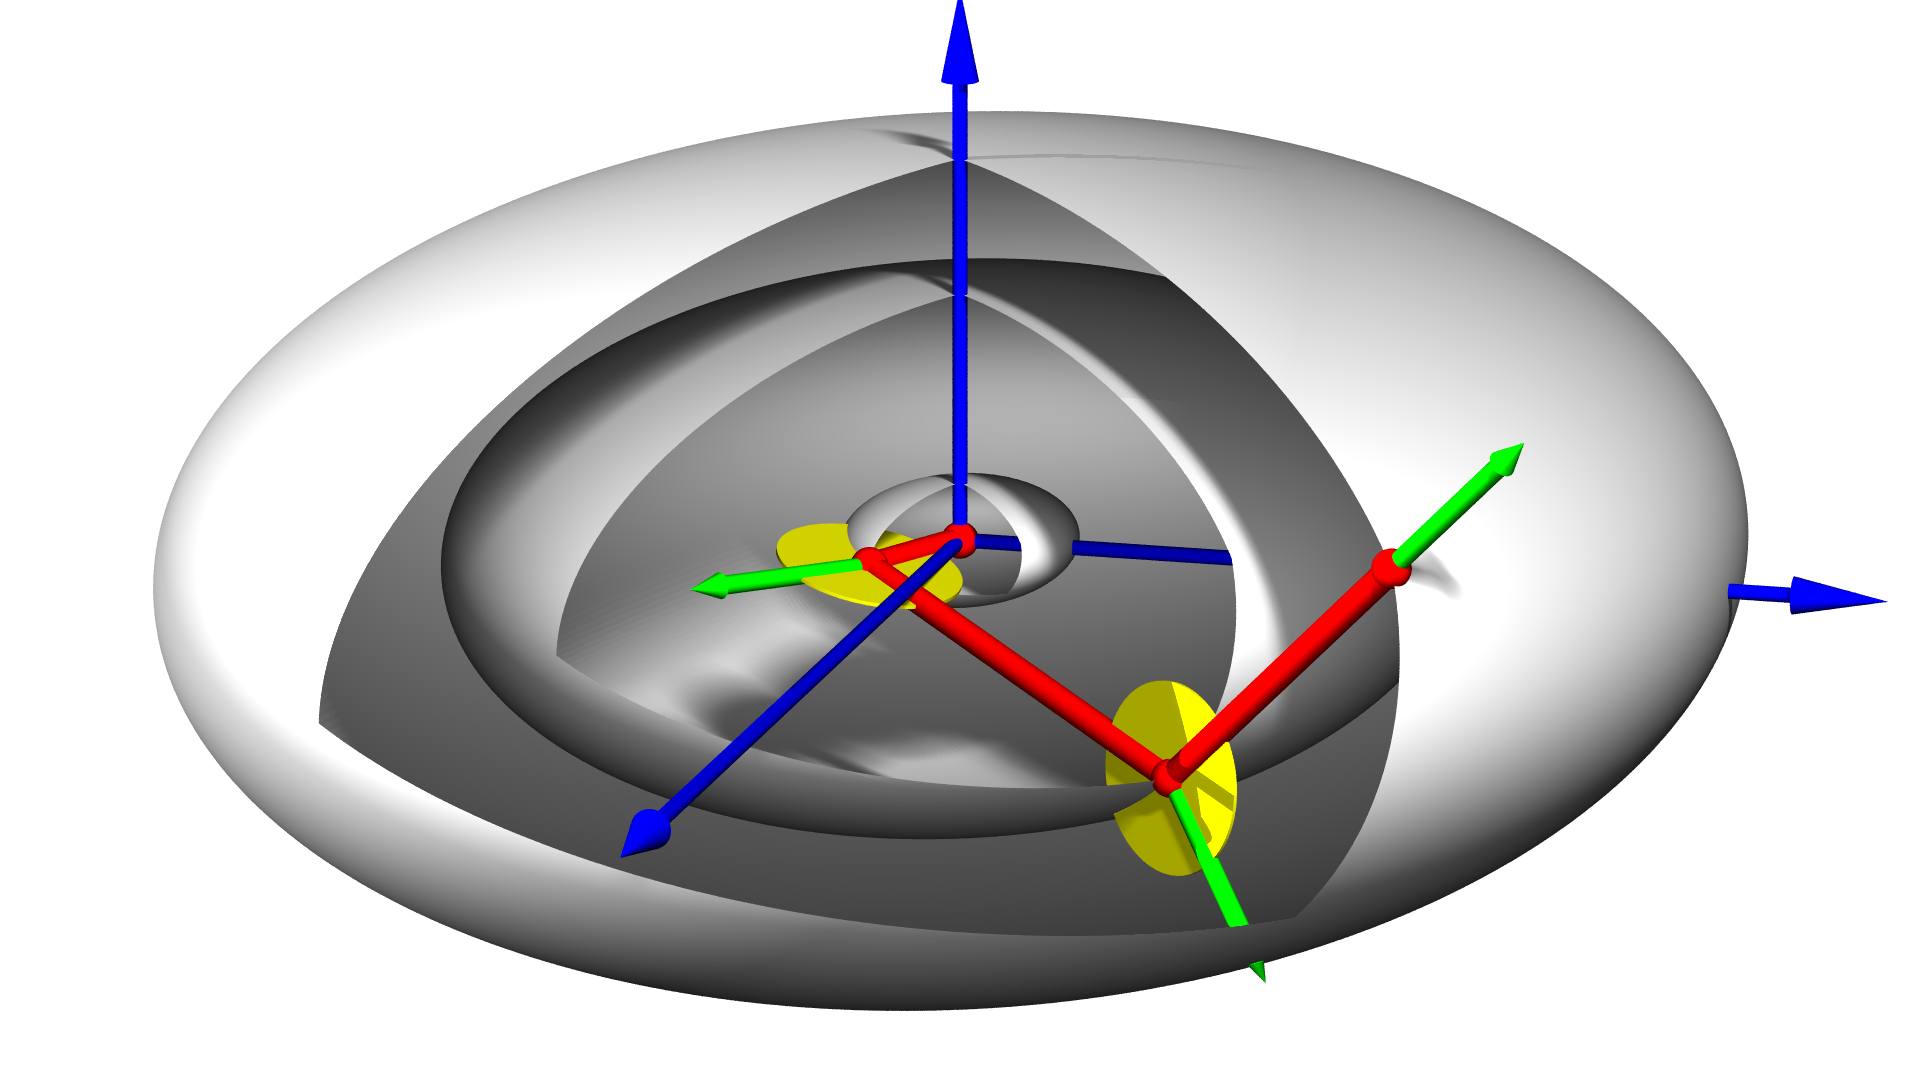
\includegraphics[width=0.8\hsize]{papers/cg/images/cg3d-large.jpg}
	\caption{3D Abstieg mit dem CG-Algorithmus, 3 Schritte genügen um die exakte Lösung zu finden. 
		Abbildung aus dem Seminar Buch von 2014 \cite{cg:book:hpc}.}
	\label{cg:abb:cg2}
\end{figure}

\subsection{Wieso genügt Orthogonalisierung auf der letzten Richtung?}
Für die Effizienz des Algorithmus ist es entscheidend, dass eine einzige Orthogonalisierung genügt.
Wieso dies funktioniert, soll hier in abgekürzter Form bewiesen werden.

\begin{proof}[Beweis]
Für den Beweis genügt es den Fall $b=0$ zu betrachten, da $b$ nur einen Offset bei der Residuumsberechnung darstellt.
Damit eine $A$-Orthogonalisierung des Residuums auf $d_k$ genügt, muss das Residuum bereits $A$-orthogonal auf den vorherigen $\langle d_1, \dots ,d_{k-1} \rangle$ Richtungen stehen
\begin{equation} \label{cg:eq:ortho1}
	r_{k+1} \perp_A \langle d_1, \dots ,d_{k-1} \rangle.
\end{equation} 
Aus dem Aufbau des Algorithmus lässt sich die Vermutung ableiten, dass die Residuen und die Richtungen den selben Raum aufspannen.
Wir nehmen also an, dass
\begin{equation}\label{cg:eq:ortho2}
\langle r_1, \dots ,r_{k-1} \rangle 
= 
\langle d_1, \dots ,d_{k-1} \rangle.
\end{equation}
Die Korrektheit dieser Annahme wird nachträglich bewiesen. 
Mit dieser Eigenschaft lässt sich die Gleichung \eqref{cg:eq:ortho1} umstellen zu
\begin{align}\label{cg:eq:ortho3}
	r_{k+1} 	&\perp_A \langle r_1, \dots ,r_{k-1} \rangle \nonumber \\
	0 			&= \langle r_{k+1}, r_i \rangle_A \quad \forall i < k-1 \nonumber\\
				&= \langle r_{k+1}, Ar_i \rangle \quad \forall i < k-1 
\end{align} 
Wir nehmen ausserdem an, dass sich die Residuen als Linearkombinationen von $r_1$ und $A$ ausdrücken lassen
\begin{equation}
	\langle r_1, \dots ,r_k \rangle = \langle r_1, Ar_1 \dots ,A^{k-1}r_1 \rangle.
\end{equation}
Auch diese Annahme wird später noch bewiesen.
Dann können wir die Menge der Vektoren $Ar_i$ aus \eqref{cg:eq:ortho3} schreiben als
\begin{align}\label{cg:eq:ortho4}
	A \langle r_1, r_2, \dots , r_{k-1} \rangle &= A \langle r_1, Ar_1 \dots ,A^{k-2}r_1 \rangle \nonumber\\
												&= \langle Ar_1, A^2r_1 \dots ,A^{k-1}r_1 \rangle \nonumber\\
												&\subset \langle r_1, Ar_1 \dots ,A^{k-1}r_1 \rangle = \langle r_1, r_2, \dots , r_k \rangle.
\end{align} 
Da der Algorithmus eine optimale Schrittweite verwendet, steht der neue Vektor $x_{k+1}$ $A$-orthogonal auf allen bisherigen Abstiegsrichtungen $d_1, \dots, d_k$.
Dieses Verhalten ist gut sichtbar in Abbildung \ref{cg:abb:cg1}.
Da $r_{k+1} = -Ax_k$ (weil $b=0$), führt die $A$-Orthogonalität von $x_{k+1}$ dazu, dass $r_{k+1}$ orthogonal auf $d_1, \dots, d_k$ steht
\begin{equation}\label{cg:eq:ortho5}
	\langle x_{k+1}, d_i \rangle_A = \langle Ax_{k+1}, d_i \rangle = \langle r_{k+1}, d_i \rangle = 0 \quad \forall i \le k.
\end{equation}
Durch Anwenden von Gleichung \eqref{cg:eq:ortho2} auf \eqref{cg:eq:ortho4} ist die Menge der Vektoren $Ar_i$
\begin{equation}
	\langle r_1, r_2, \dots , r_k \rangle = \langle d_1, d_2 \dots ,d_k \rangle.
\end{equation} 
Wenn wir dies mit Gleichung \eqref{cg:eq:ortho5} vergleichen, sehen wir dass dadurch die Bedingung aus Gleichung \eqref{cg:eq:ortho3} erfüllt ist.
Somit ist die Anfangsvermutung $r_{k+1} \perp_A \langle d_1, \dots ,d_{k-1} \rangle$ bewiesen.
\end{proof}

In diesem Beweis haben zwei Teile gefehlt, welche nun noch nachträglich bewiesen werden.
Das erste wäre die Annahme, dass die Residuen und die Richtungen den selben Raum aufspannen $\langle r_1, \dots ,r_{k-1} \rangle = \langle d_1, \dots ,d_{k-1} \rangle$.

\begin{proof}[Beweis]
Wir beginnen damit den Algorithmus für die Berechnungen von $d_k$ aufzuschreiben (vgl. Gleichung \eqref{cg:eq:gram})und erhalten
\begin{align}
	d_1 &= r_1 \nonumber\\
	d_2	&= r_2 - a_2 d_1\nonumber\\
	d_3	&= r_3 - a_{31} d_1 - a_{32} d_2\nonumber\\
	d_k &= r_k - \sum_{i=1}^{k-1} a_{ki} d_i.
\end{align}
Durch Umstellen nach $r_k$, sieht man dass $r_k$ aus $\langle d1, d2, \dots, d_k \rangle$ linear kombiniert werden kann.
Dasselbe macht man für $d_k$, wobei $d_i$ mit $i<k$ aufgelöst wird bis $d_1 = r_1$.
Daraus folgt dass auch $d_k$ aus $\langle r_1, r_2, \dots, r_k \rangle$ linear kombiniert werden kann.
Somit ist $\langle r_1, \dots ,r_{k-1} \rangle = \langle d_1, \dots ,d_{k-1} \rangle$ bewiesen.
\end{proof}

Das zweite wäre die Annahme, dass sich die Residuen als Linearkombinationen von $r_1$ und $A$ ausdrücken lassen $\langle r_1, \dots ,r_k \rangle = \langle r_1, Ar_1 \dots ,A^{k-1}r_1 \rangle$.

\begin{proof}[Beweis]
Wir beginnen wiederum damit, den Algorithmus aufzuschreiben (diesmal für $r_k$) und erhalten
\begin{align}
	r_1 &= -Ax_1 \\
	r_2	&= -Ax_2 = -A(x_1-r_1) = Ar_1 - r_1 \nonumber\\
	r_3 &= -Ax_3 = -A(x_2-r_2) = Ar_2 - r_2 \nonumber\\
	r_k &= Ar_{k-1} - r_{k-1} \in \langle r_1, Ar_1, \dots, A^{k-1}r_1 \rangle.
\end{align}
womit diese zweite Annahme bereits bewiesen wäre.
\end{proof}

Eine noch ausführlichere Variante dieses Beweises findet sich im Dokument \cite{cg:online:cgmueller}.

	
